\documentclass[11pt]{article}
%Gummi|063|=)
\usepackage{graphicx}
\usepackage{amsmath}
\usepackage[lofdepth,lotdepth]{subfig}
\usepackage{multirow}

\title{\textbf{Applied Econometric Projects Seminar draft of results}}
\author{Johannes Degn}
\date{01.07.2013}
\begin{document}

\maketitle

\section{Haystacks}

We have been given 3 different data sets with a y variable and 40, 40 and 57 x variables respectively for data set 1, 2 and 3.
Figures \ref{correlograms1}, \ref{correlograms2} and \ref{correlograms3} show scatterplots between y and the covariates. The first data set features 40 covariates where each covariate is moderately correlated with y. They appear to be comming from a similar data generating process (with possibly different distributional parameters).
The second data set contains 40 covariates of which 5 are strongly correlated with y and the rest show no visible correlation with y. It looks like there are at least two underlying data generating processes.
The last data set is the most complicated one on first view. It contains 56 covariates for which no clear patterns can be made out on first sight regarding the correlation with y. It looks like there are 3 data generating processes. The most interesting variable is $X_{57}$ which has no negative values. It turns out that $X_{57}$ is just $X_{10}$ squared\footnote{credit goes to my colleague, Stefan Voigt for finding this gem}.

\section{Approaches}

\subsection{OLS}
Given the information given about the correlations of ys and xses, it is evident that OLS will perform best for data set 2. Here we have several variables with a high correlation with y. Resultingly figure \ref{ols2} shows a very tight fit both in and out of sample. While this result is tough to beat for this data set, Best Subset seems to achieve better out of sample forecasts.
\subsection{Best Subset}
\subsection{Targeted Predictors (Bai \& Ng 2008)}
\subsection{Lasso}
\subsection{LAR}
\subsection{Ridge}
\subsection{Random Forests}

\begin{figure}
\caption{correlation of y with the xses - data set 1}
\label{correlograms1}
\centering
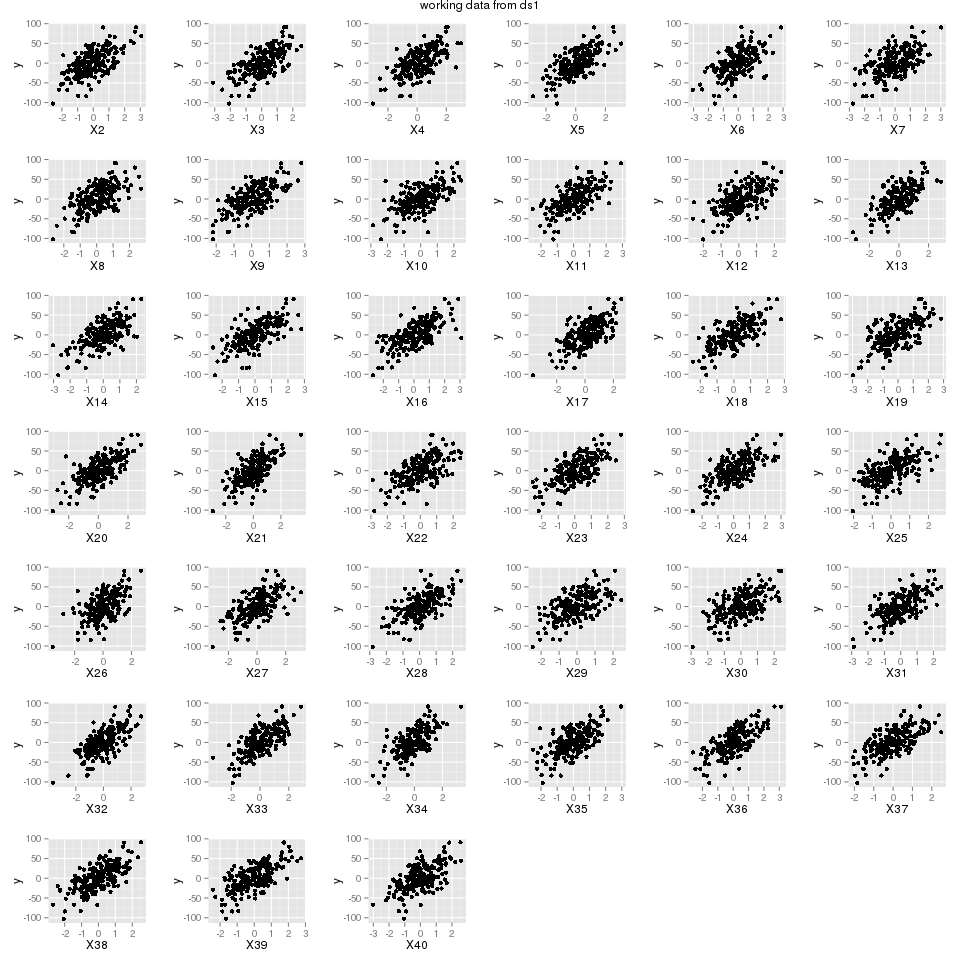
\includegraphics[width=100mm]{graphs/correlograms1.png}
\end{figure}

\begin{figure}
\caption{correlation of y with the xses - data set 2}
\label{correlograms2}
\centering
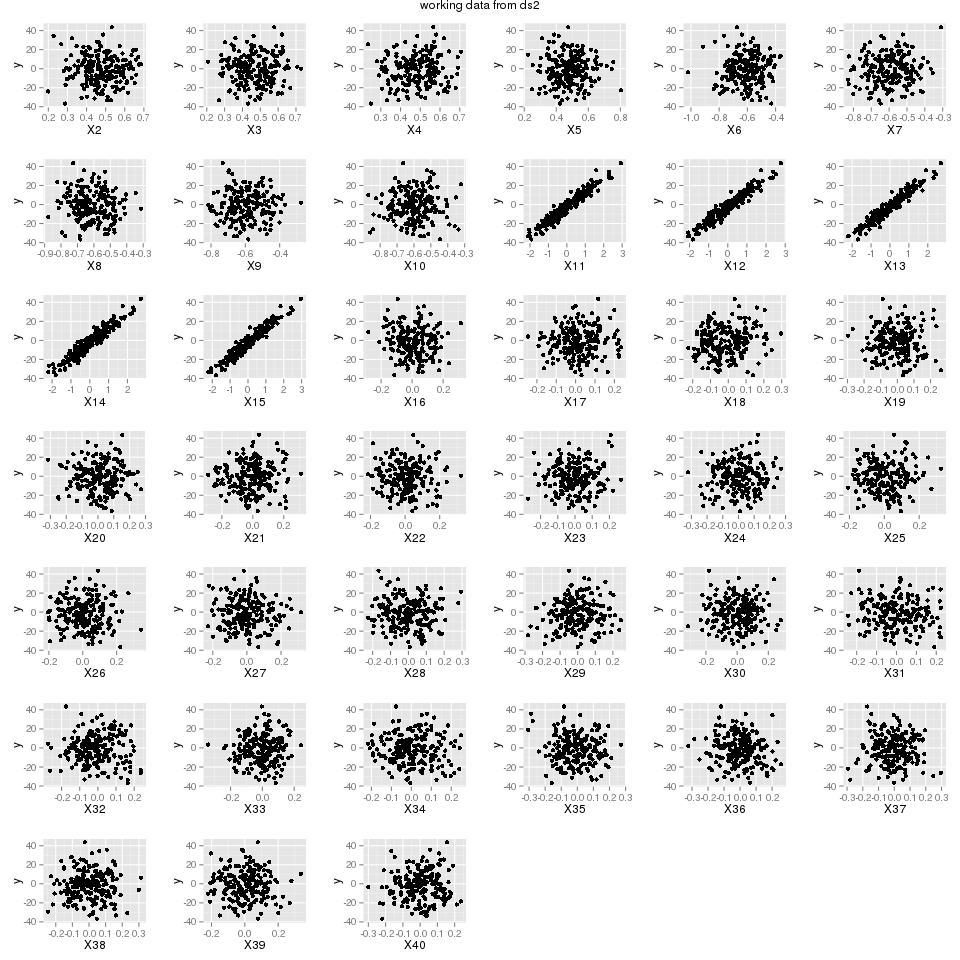
\includegraphics[width=100mm]{graphs/correlograms2.png}
\end{figure}

\begin{figure}
\caption{correlation of y with the xses - data set 3}
\label{correlograms3}
\centering
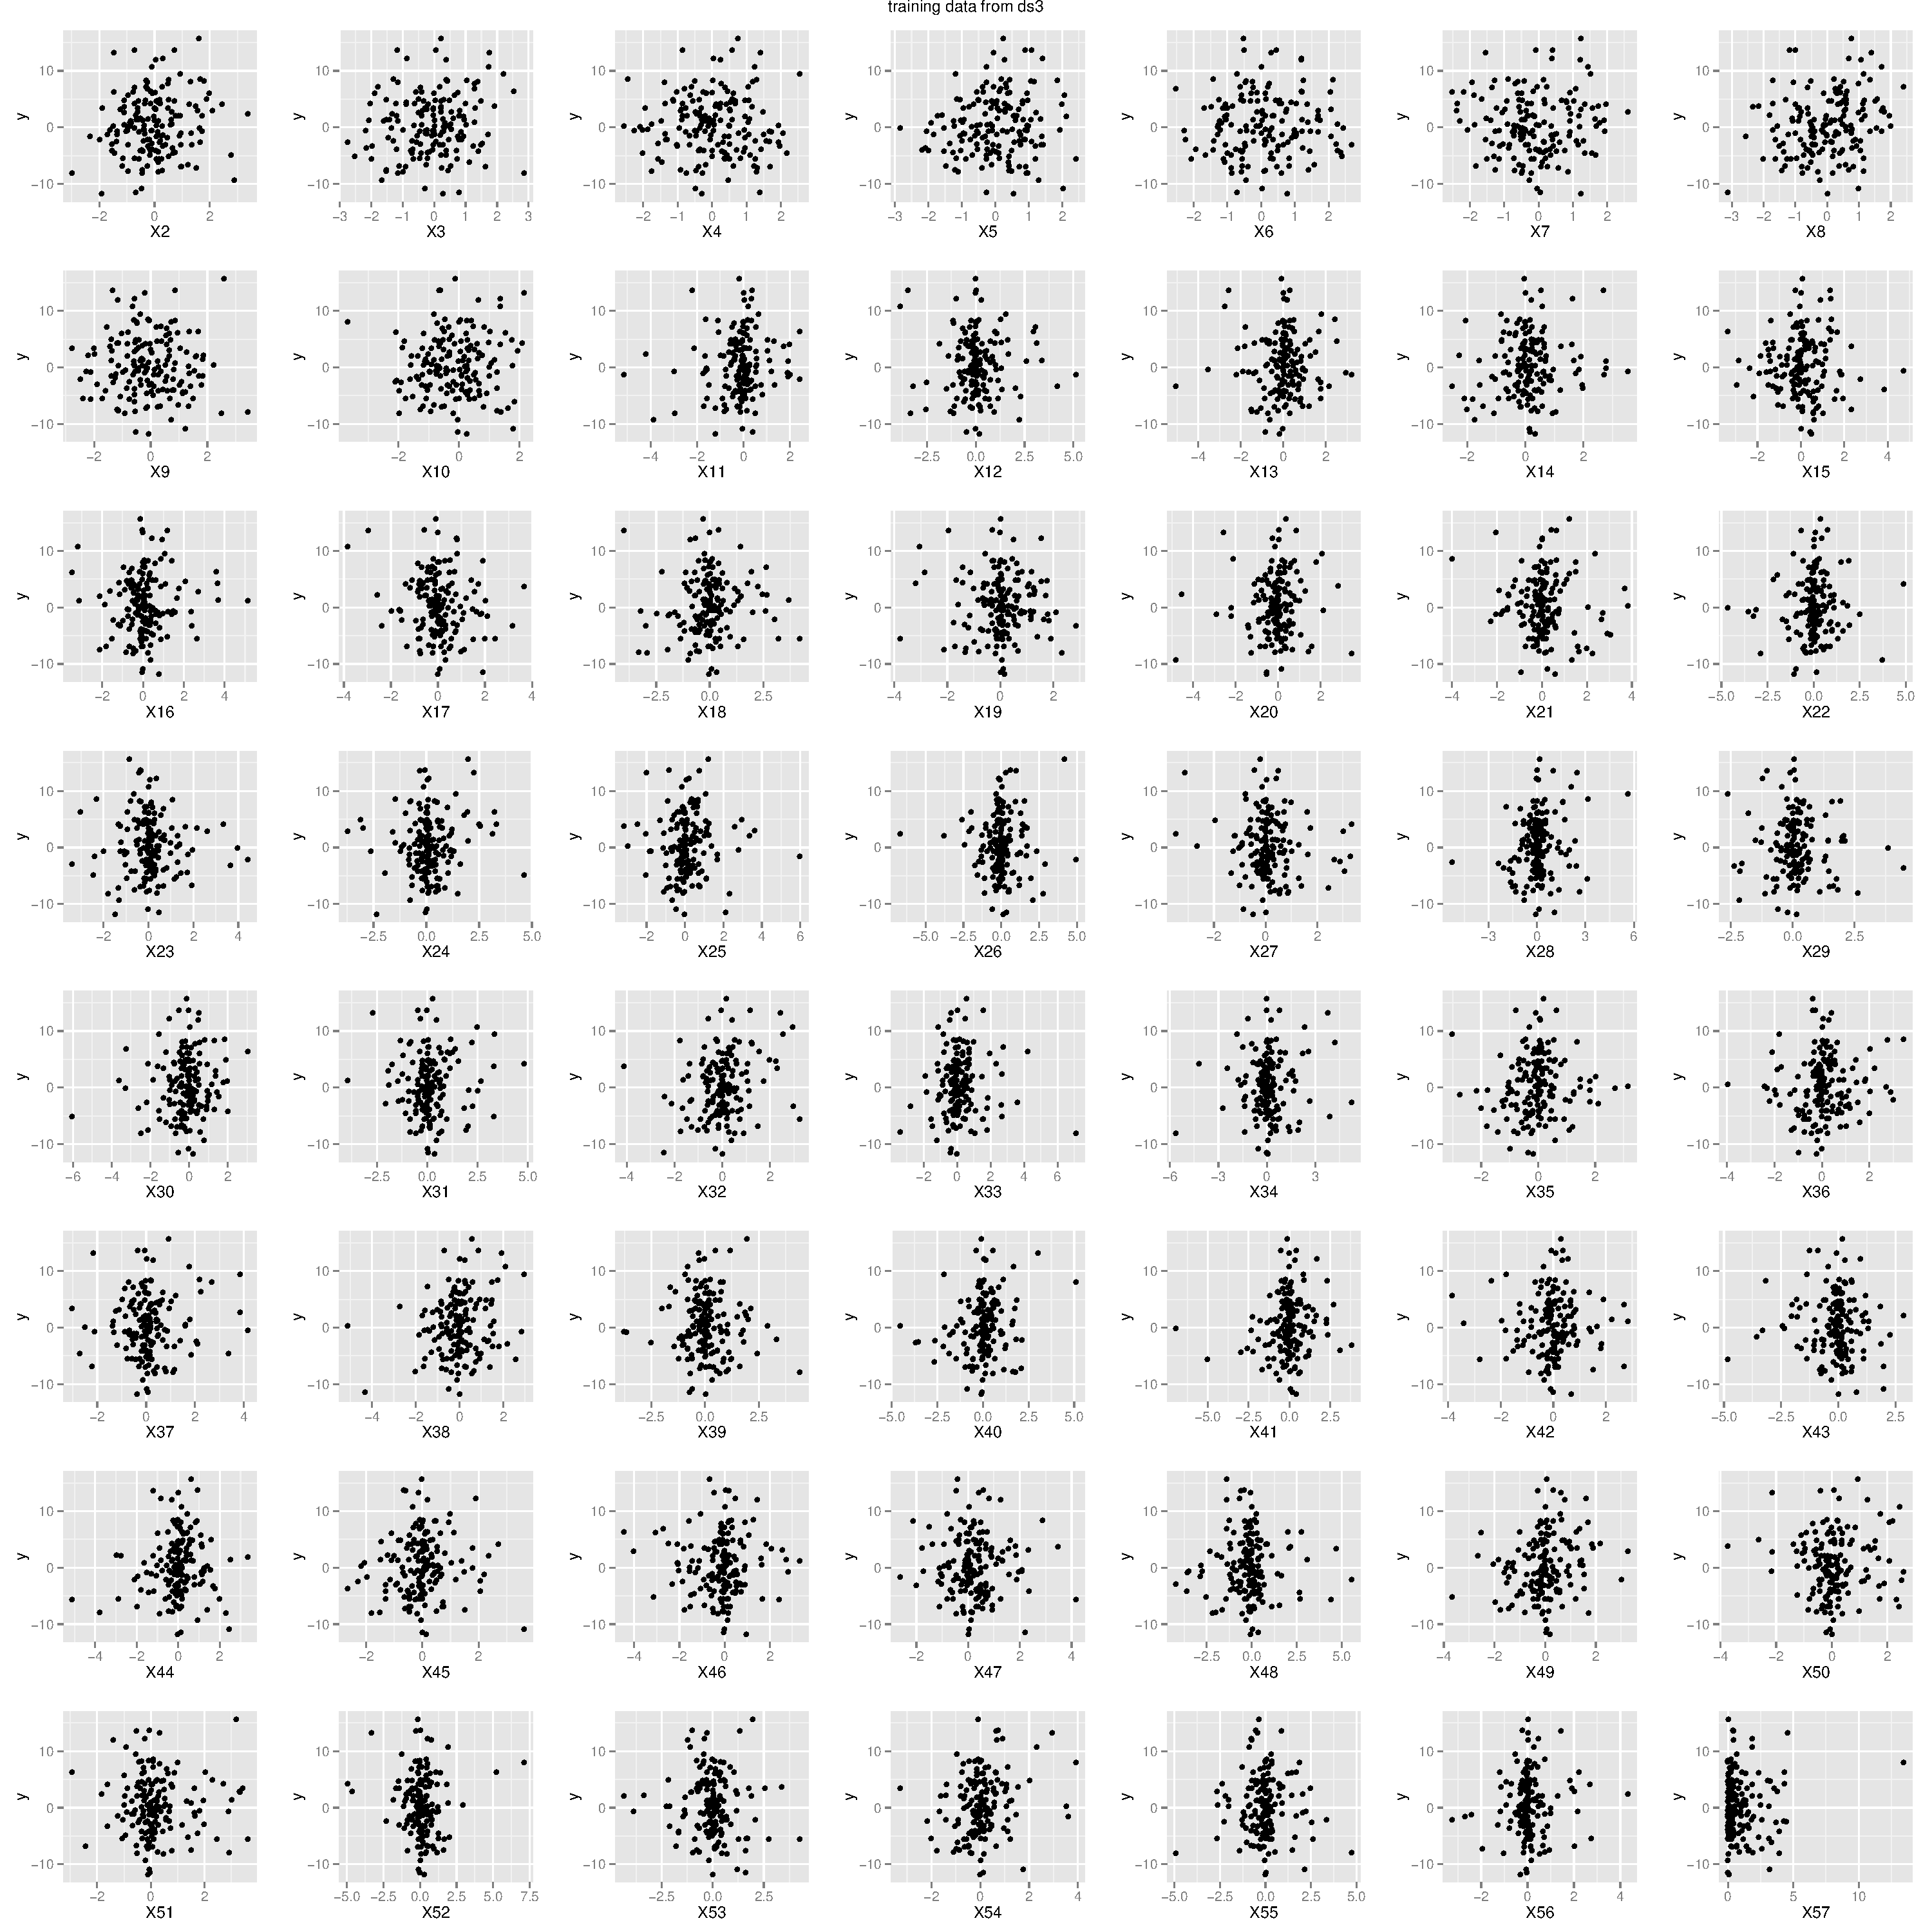
\includegraphics[width=100mm]{graphs/correlograms3.pdf}
\end{figure}

\begin{figure}
\caption{OLS - data set 2 (160 training and 40 validation observations)}
\label{ols2}
\centering
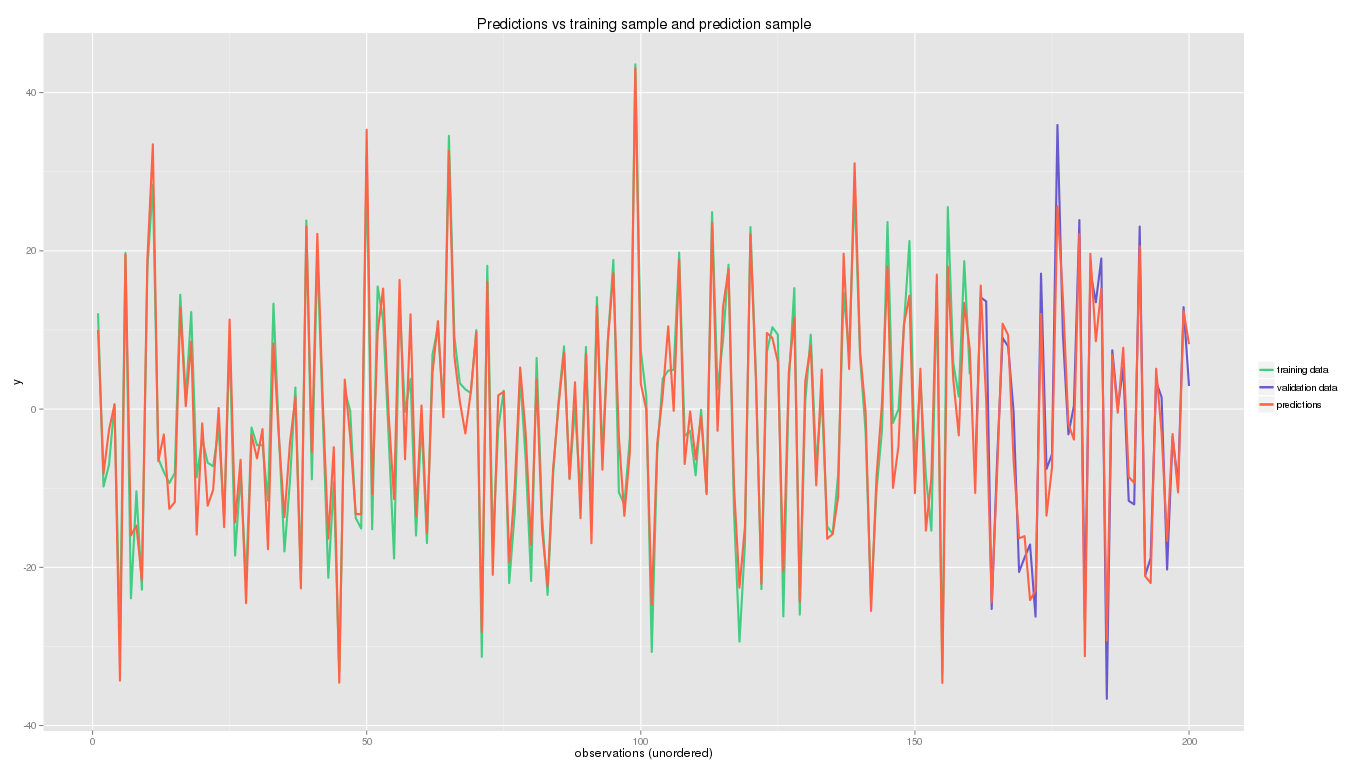
\includegraphics[width=100mm]{graphs/ols2_validation.png}
\end{figure}

\begin{table}[hc]
\caption{Out of sample mses, k-folded (k=5, 20 repetitions)}
\label{mses kfolded}
\begin{tabular}{l|ccc}
Data Set & OLS & Best Subset & Targeted Predictors \\
\hline
1 & OLS & Best Subset & Targeted Predictors \\
2 & OLS & Best Subset & Targeted Predictors \\
3 & OLS & Best Subset & Targeted Predictors \\

\end{tabular}
\end{table}


\end{document}
